% Chapter 6

\chapter{Automated Reconfiguration}
\label{Chapter 6}
\lhead{}

% 1 . Overview - what is the purpose of an agent?
\section{Overview}
This chapter discusses automated network reconfiguration and how it is supported by the work of this thesis. First, the concept of automated reconfiguration and the motivation for its use is described. Then the design and implementation of the automated reconfiguration software in the work of this thesis is described. Finally, an example is shown that demonstrates the practical uses of this software.

% 2. Design 
%	- describe automated user & message processor 
%	- message processor is what distinguishes one agent from another 
%		- message processor can be made with a lambda and passed around as a first-class object (treating a function as a variable)
%		- cite this concept of lambda as a first class object
%	- the need to validate and separate permission checking from the automated user
%		- provides the motivation for a agentController
%	- mention how automated user is using the same logic/code from earlier in the paper
%		- using the same command classes
%		- automation is a natural extension of the work in the previous chapters
%	- class diagram of how all the classes fit together

\section{Requirements}
The work in this thesis allows network reconfiguration through user interaction. User interaction can sometimes be inadequate because of slow response time, a lack of understanding of system behavior, or human error. Creating a system that can automatically respond to incoming sensor data (or calculations derived from incoming sensor data) by reconfiguring the network overcomes many limitations encountered by requiring user input.


% 1. Describe the automated user class and how it needs to support several things when new automated users are implemented:
% - be able to handle received messages and exceptions that may be encountered
% - be able to adhere to the user access and safety validations of the rest of the system
% NOT allow some automated users to overwrite the UAC and safety validation
% NOT directly interact with the database
The software applications designed in this work to autonomously monitor and reconfigure WiSARDs are called automated agents. Agents must fulfill three main requirements. First, the agents must adhere to the user access and safety validations that govern the rest of the system. More specifically, the developers of automated agents should not be allowed to intentionally or unintentionally bypass, improperly implement, or override the security provisions. Second, they must be able to receive and handle WiSARD data streams as well as any exceptions that may occur. WiSARD data streams are accessible to applications by using an MQTT subscription client. These data streams are called messages. Finally, the agents should be able to interact with the other CI systems. For instance, an agent should be able to interact with the PostgreSQL database using the query methods that the WiSARD class provides.

\section{Design}
The automated agents are defined by a Java class designed to address these requirements. The first requirement of preventing agents from circumventing system security is solved by separating the validation logic from the Agent Class. If the validation logic is external to the Agent Class, then agents will not be able to dictate their own security privileges. The second requirement of receiving and handling data streams and handling exceptions specific to each agent is solved by the design decision that each agent has message handling logic and exception handling logic that can be specific to that agent. The final requirement of allowing an agent to interact with the other parts of the CI  is solved by using the functionality in Wisard\_Browser\_Module, Cmd\_Generation\_Module, and Validation\_Module. For instance, an agent can use the WiSARD Class discussed in Chapter 5 as a means of interacting with the database.

To implement this design, the AgentController Class is used and encapsulates much of the functionality described in the previous chapters, primarily validation and safety. The controller class will log in an agent, validate that it has sufficient privileges to access the data streams it uses, and then create an agent object. The agent class implements the Java runnable interface, allowing the agent to be put into a thread and executed. The design and implementation of the agents is generalized, so that there is common code from agent to agent. Every agent uses the same logic to listen for and handle incoming messages. Message processing and error logic that distinguishes one agent from another are passed to the agent as parameters in the form of lambda expressions (anonymous functions).

Using inheritance in object-oriented software design is typically a good way to reuse code. Inheritance has been used extensively in the code described in the previous chapters. However, in the case of designing the automation behavior, using aggregation over inheritance resulted in a cleaner design. Aggregation is the object-oriented design concept where the functionality of an object is determined by the aggregation of other objects, as opposed to implementing or inheriting the functionality directly. This approach is accomplished with the use of two interfaces referred to as the MessageProcessor and the ErrorHandler. These interfaces allow the operational logic for each agent to be passed in as lambda expressions to an Agent object during its creation. Figure \ref{fig:automation_class_diagram} is a UML class diagram that shows how agents are implemented using aggregation.

\begin{figure}[H]
	\centering
	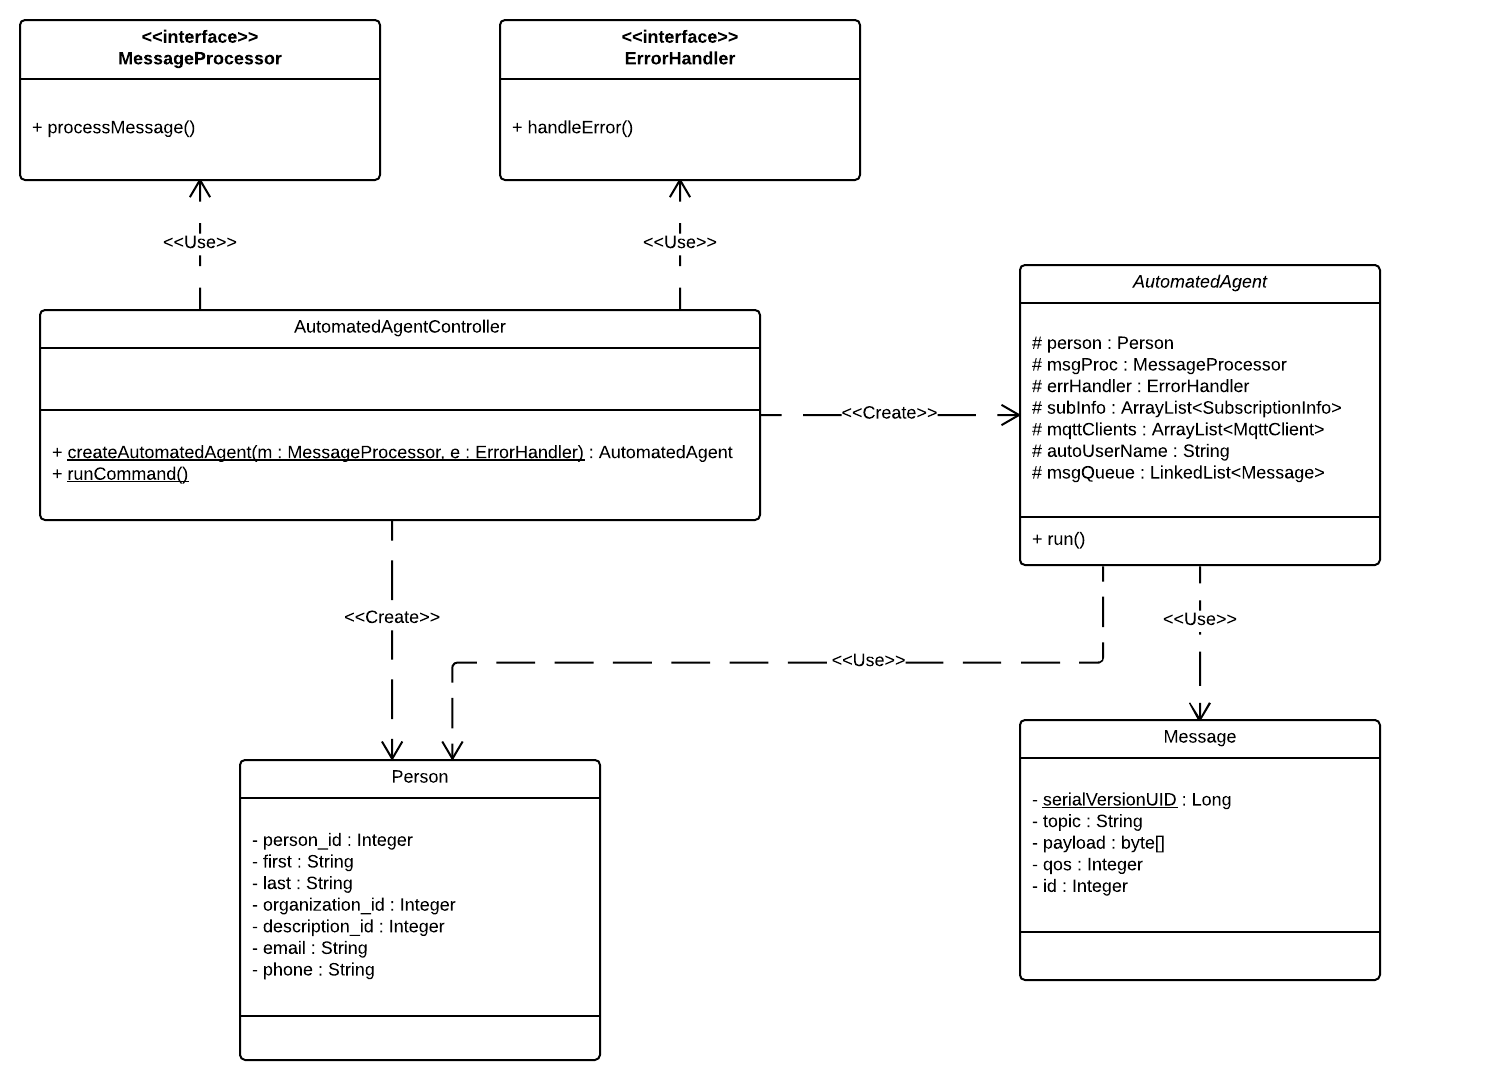
\includegraphics[width=\textwidth]{figures/automated_agent_class_diagram.png}
	\caption{A UML class diagram showing the classes and interfaces necessary to instantiate AutomatedAgent objects. The arrows describe the relationships between the four different classes as well as the two interfaces. }
	\label{fig:automation_class_diagram}
\end{figure}

AutomatedAgentController, AutomatedAgent, Person, and Message are each a class. MessageProcessor and ErrorHandler are functional interfaces. A functional interface defines a type for a lambda expression. This is necessary so that variables can be created to reference lambda expressions.  The text on each of the arrows describes the relationship between the classes and interfaces used in the automation software. The AutomatedAgentController class \verb|<<uses>>| the MessageProcessor and ErrorHandler interfaces to store lambda expressions that implement the logic for processing messages and for handling errors, respectively.

The AutomatedAgentController class \verb|<<create>>| instances of both the Person class and the AutomatedAgent class. An AutomatedAgentController takes in the two lambda expressions, creates a Person object, and passes those along into the constructor of AutomatedAgent class to create new agents. 

Each AutomatedAgent object can then use its Person object, the functionality in the Message class, and whatever lambda expressions that were passed in as the MessageProcessor and ErrorHandler. A detailed example of the software classes showing how this software works is described in the next section.

\section{Example Agent}
% 3. Example description and code for a very simple agent
%	- flow of execution visual?%
Using the design described in the previous section, there are many different ways that an automated agent can be used to manage WiSARDs. The following code snippets demonstrate how this software is used in practice by showing the class definitions for AutomatedAgentController and AutomatedAgent, the definitions for the MessageProcessor and ErrorHandler functional interfaces, as well as an example program which demonstrates how to use these classes.

Below is a simplified class definition for the AutomatedAgentController class that handles authentication, creation, and execution of the agents.
% AutomatedUserController class
\lstinputlisting[language = java, firstline = 32, lastline=44]{AutomatedUser.java}
 
The code snippet shown below contains the definitions for the functional interfaces that allow lambda expressions to be passed to the agents that define their behavior. A type is a notation that specifies how variables or objects should be interpreted and used. As described in the previous section, functional interfaces specify a type that allows lambda expressions to be saved to variables and used by the agents. In the case of these interfaces, the types are MessageProcessor and ErrorHandler. 

 % Interfaces
 \lstinputlisting[language = java, firstline = 16, lastline=30]{AutomatedUser.java}
 
The snippet shown below is the class definition for AutomatedAgent. In the constructor, all necessary information to establish connections to MQTT message brokers as well as define the agent's behavior is passed in as a set of parameters. The method \verb|run()| establishes its subscriptions with the MQTT brokers it will be listening to, and then waits for messages to arrive. Once messages arrive, they are given to \verb|processMessage()| whose functionality was passed into the constructor as a lambda expression. Additionally, any exceptions are passed to \verb|handleError()| whose functionality was also passed to the constructor as a lambda expression.

%\lstinputlisting[language = java, firstline = 46, lastline=62]{AutomatedUser.java}
  
 % AutomatedUser class	
 \lstinputlisting[language = java, firstline = 64, lastline=132]{AutomatedUser.java}
 
 The final code snippet below shows a simple example of how to utilize the classes defined above in an agent that automatically reconfigures a WiSARD. This example program creates an agent that toggles between two different sampling rates every 12 hours. The \verb|main()| method shown at the bottom of this example uses the AutomatedAgentController class to instantiate an AutomatedAgent object with the \verb|createAutomatedAgent()| method. Note that no instance of the AutomatedAgentController class created. This is because the method is declared to be static. Likewise, \verb|runCommand()| is also static. The Java Virtual Machine (JVM) allows static methods to be called without creating an instance of the class that defined them.
 
 \lstinputlisting[language = java, firstline = 7, lastline = 79]{Agent_example.java}
 
 \section{Greenhouse Experiment}
To demonstrate the ability of the automated agent framework described in this chapter, an experiment was devised and an agent created to automatically manage the experiment parameters. 

% 6.4.1 Setup the experiment
\subsection{Setting up the Experiment}
A WiSARD network was deployed to a site at Northern Arizona University. This site is located within a greenhouse containing buckets with various soil types. Each bucket has holes in the bottom along with a mesh fabric, allowing water to drain out of the buckets, but not the soil. Over each bucket is a water line with a 1/2 gallon per hour drip emitter that regulates the amount of water a bucket receives from a water line. A WiSARD with a SP-CM-STM controls the watering events by actuating a latching solenoid water valve. Additionally, a separate WiSARD with a Decagon 5TM transducer is monitoring the dielectric permittivity of the soil at a depth of 20cm. Dielectric permittivity is an important measurement that can be used to determine the volumetric water content (VWC) of a soil. Finely ground cinders from Northern Arizona were chosen as the soil for this experiment.

The objective of the experiment is to maintain the dielectric permittivity at a depth of 20cm between an upper and a lower threshold. The Decagon 5TM transducer measure dielectric permittivity in a raw version which needs to be converted to the true dielectric permattivity. The conversion is \[ \varepsilon_{a} = \varepsilon_{raw} / 50 \] 

The Decagon 5TM can measure raw dielectric permittivity on a scale of 1 (completely dry) to 4000 (completely wet). To maintain the maximum sampling resolution, the control is maintained by acting upon raw transducer measurements as opposed to the final values for dielectric permittivity. The agent controls the levels by turning the water valve on and off such that the dielectric permittivity is kept between 400 and 520. Since the transducer is buried at a depth of 20cm, there is a latency between when the moisture exits the waterline and when it is sampled by the transducer. There is also network latency both when sending a command to a WiSARD and receiving a sample value from the WiSARD. For these reasons, threshold values of 410 and 480 were chosen to compensate for the described latencies. The lower threshold requires less compensation than the upper threshold due to slow rate at which it dries. 

% 6.4.2 Agent Implementation
\subsection{Agent Implementation and Results}
The specific agent used to control this experiment follows the framework described in the previous section. The control logic which this agent follows is shown in \ref{fig:agent_logic}. The agent is a multi-threaded command line Java program. The main thread of the agent program creates the agent object using the classes and methods described in the previous sections of this chapter. The agent is then executed in a separate thread; it receives and processes messages from the sampling WiSARD and sends out reconfiguration commands using the ActuateValve command class mentioned in chapter 5.

% logic diagram figure
\begin{figure}[H]
	\centering
	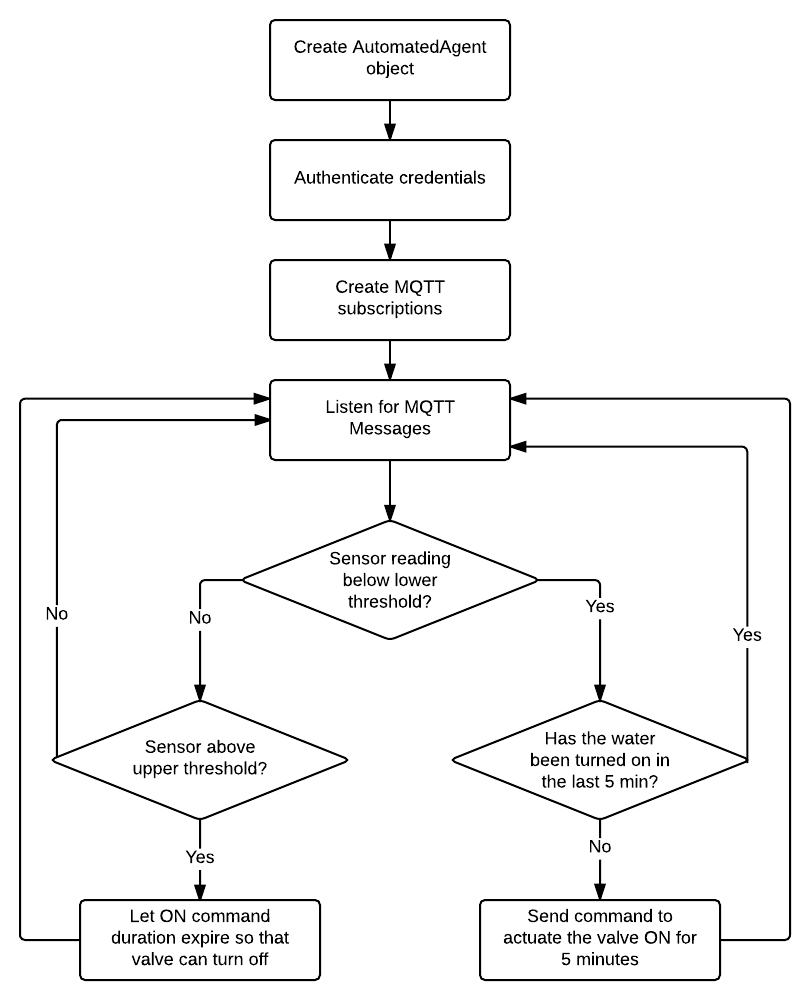
\includegraphics[width=.8\textwidth]{figures/greenhouse_agent_logic.png}
	\caption{The automated agent that controls the greenhouse experiment follows this logic diagram.}
	\label{fig:agent_logic}
\end{figure}

The core logic of the agent's control algorithm is implemented in a MessageProcessor lambda expression. The following code segment shows the MessageProcessor for this agent in its entirety. The logic in the MessageProcessor is what the agent executes whenever a new message is received. Each message is parsed and analyzed to determine whether it contains a sample from the transducer at a depth of 20cm. A WiSARD reports many streams, and samples from different transducers often are grouped into the same message in the WiSARD wireless communication protocol. If a message is obtained containing a sample from the transducer of interest, the logic in the MessageProcessor will use the measurement to determine whether the valve should be turned on.

% code listing for greenhouse agent message processor
\lstinputlisting[language = java, firstline = 1, lastline=83]{message_processor.java}

If the dielectric permittivity level is determined to be less than the lower threshold value, the ActuateValve command class is used to synthesize a command message which will instruct the WiSARD to actuate the valve into the open state for a five minute duration. When the time parameter in a valve duration command message expires, the WiSARD will actuate the valve into the closed position, stopping the flow of water into the bucket. If another valve actuation command is sent to a WiSARD while there is still time remaining from the previous command's duration, the value of the remaining time is overwritten with the duration parameter of the new command message. The software in this MessageProcessor continually sends valve actuation command messages with five minute durations for as long as the transducer reports readings less than the upper threshold. If the upper threshold is passed, then the duration is allowed to expire and no more messages are sent until the samples once again fall below the lower threshold.

Figure \ref{fig:control} shows the raw dielectric permittivity samples from the Decagon 5TM transducer while the agent was active. The green dashed lines indicate the threshold values of 410 and 480 used to actuate the valves. The red regions indicate the periods where the valves were open and allowed water to flow into the soil. The agent ensured that the raw dielectric permittivity never exceeded 520 nor did it fall below 400. 

\begin{figure}
	\centering
	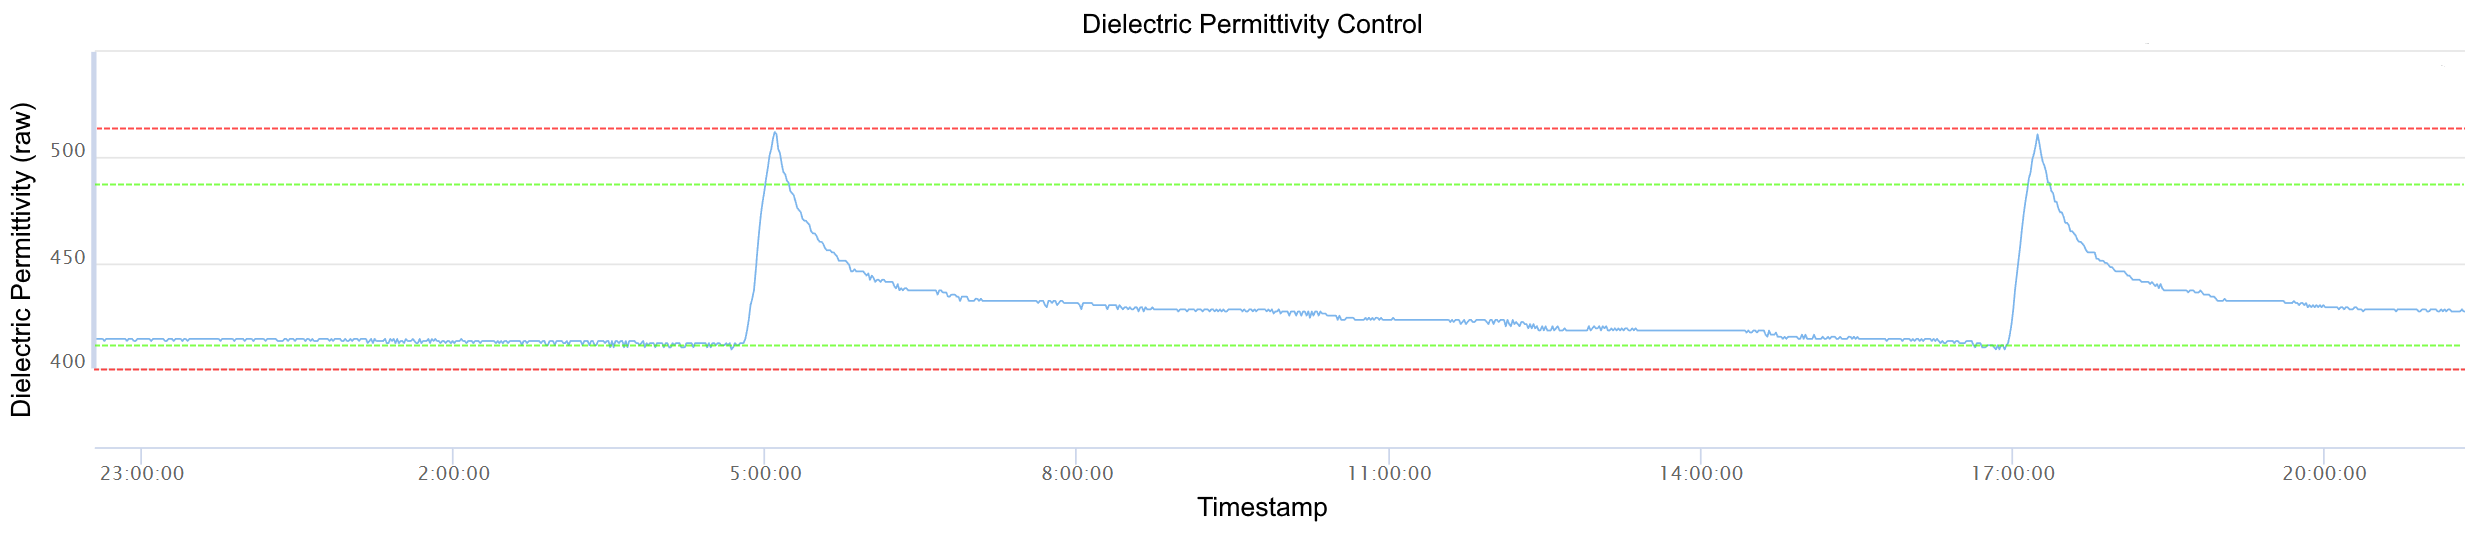
\includegraphics[width=\textwidth]{figures/moisture_control_portal_edit.png}
	\caption{}
	\label{fig:control}
\end{figure}

% 6.5
\section{Summary}
Automated reconfiguration is a valuable feature that allows for greater control over a WSN. The automated agent software framework described in this chapter allows automated reconfiguration to be utilized in WiSARDNet. The greenhouse control experiment demonstrates the ability of an automated agent to control an experiment on a live WiSARD network by utilizing the software modules described in Chapter 5. A user can utilize this software framework to create their own automated agents. Appendix \ref{appendix:guide} provides instructions on how to create an automated agent.


